% Chapter Template

\chapter{Resultados} % Main chapter title

\label{Chapter5} % Change X to a consecutive number; for referencing this chapter elsewhere, use \ref{ChapterX}

%----------------------------------------------------------------------------------------
%	SECTION 1
%----------------------------------------------------------------------------------------

Este capítulo muestra algunos de los resultados obtenidos por el método experimental presentado en el capítulo anterior.

\section{Discusión de resultados obtenidos}

A continuación se describirán los resultados por cada etapa del método experimental.

\subsection*{Obtención de datos y procesamiento}

Para obtener el conjunto de datos, primero se optó por intentar generar una base de datos usando el simulador CORSIKA, sin embargo, se observo que la generación de un dataset de al menos $60000$ observaciones, tomaría un tiempo inviable con el equipo de cómputo con el que se disponía. Del mismo modo, la complejidad adicional que la interfaz del programa y la inexperiencia con el mismo, agregaba una dificultad extra a la hora de configurar los parámetros del evento. 

Por consiguiente, se decidió buscar una base de datos de simulaciones que estuvieran disponibles al público. De modo que el banco de datos que se usó fue tomado de \parencite{Erdmann2018b}, el cual contiene $100000$ simulaciones de cascadas electromagnéticas (Tabla~\ref{tab:DBfeatures}).

\begin{table}
    \caption{Parámetros de la base de datos.}
    % $N=100000$
    \label{tab:DBfeatures}
    \centering
    \begin{tabular}{l l l}
        \toprule
        \textbf{Etiqueta} & \textbf{Descripción} & \textbf{Dimensión} \\
        \midrule
        showermax & Coordenadas del máximo de la cascada & $(N,3)$\\
        time & Tiempos de arribo al detector $i$ & $(N,9,9,1)$\\
        Xmax & Altura de desarrollo máximo & $(N,)$\\
        signal & Contador de particulas en detector $i$ en $80$ intervalos de tiempo & $(N,9,9,80)$\\
        logE & Energía de la partícula primaria & $(N,)$\\
        showeraxis & Coordenadas del eje de la cascada & $(N,3)$\\
        showercore & Coordenadas del núcleo de la cascada & $(N,3)$\\
        mass & Masa de la partícula primaria & $(N,)$\\
        detector & Coordenadas del detector $i$ & $(81,3)$\\
        \bottomrule\\
    \end{tabular}
\end{table}

Para la selección y preprocesamiento de datos se seleccionó la señal que contiene los tiempos de arribo y la energía asociada a cada cascada. Después se hizo el ajuste propuesto en \parencite{Erdmann2018b} a los tiempos de arribo \ref{eq:proposedTimeTrans}, sin embargo el ajuste no lograba un buen entrenamiento, así que se hizo un mapeo lineal al dominio $[1,2]$.

\begin{equation}
    \label{eq:proposedTimeTrans}
    \tilde{t}_{0,i} = \frac{t_{0,i} - \tau_{evento}}{\sigma_{t,datos}}
\end{equation}

\addFigure{Figures/timesignals.png}{timesignals}{Datos de entrenamiento}{
    Gráficas de $4$ eventos detectados por un arreglo de detectores con $1000$ \textit{m} de separación entre ellos, con su respectiva energía.
}

Para el escalar de la energía de cada cascada, se decidió categorizar la variable continua en $4$ rangos energéticos, los cuales son $[(18.499, 18.875] < (18.875, 19.25] < (19.25, 19.625] < (19.625, 20.0]]$.

\subsection*{Modelo y entrenamientos}

Para la arquitectura de los modelos se optó por usar capas convolucionales, con el fín de preservar la información entre detectores. Para una descripción mas detallada de cada arquitectura revisar \textbf{Anexo \ref{AppendixA}}.

El único parámetro que se modificó fue la dimensión del vector latente (Table~\ref{tab:modelhyperparameters}), y se guardaron los modelos resultantes para cada dimensión, sin embargo se observó que para dimensiones bajas el modelo llegaba a un colapso de modos con más frecuencia (Table~\ref{tab:latentDimTrains}).

\begin{table}
    \caption{Parámetros de la base de datos.}
    % $N=100000$
    \label{tab:latentDimTrains}
    \centering
    \begin{tabular}{l l l}
        \toprule
        \textbf{Nombre} & \textbf{Dimensión} & \textbf{Frecuencia} \\
        \midrule
        cwagn\_ld4\_Ri\_checkpoint.pth.tar     & 4    & 1/4\\
        cwagn\_ld8\_Ri\_checkpoint.pth.tar     & 8    & 1/3\\
        cwagn\_ld16\_Ri\_checkpoint.pth.tar    & 16   & 1/2\\
        cwagn\_ld32\_Ri\_checkpoint.pth.tar    & 32   & 1/2\\
        cwagn\_ld64\_Ri\_checkpoint.pth.tar    & 64   & 1/1\\
        cwagn\_ld128\_Ri\_checkpoint.pth.tar   & 128  & 1/1\\
        \bottomrule\\
    \end{tabular}
\end{table}
%insertar gráficas de pérdidas en el entrenamiento.

\subsection*{Generación de cascadas electromagnéticas}

\begin{table}
    \caption{Parámetros del modelo.}
    \label{tab:modelhyperparameters}
    \raggedleft
    \begin{tabular}{l l l}
        \toprule
        \textbf{Nombre} & \textbf{Descripción} & \textbf{Valor inicial} \\
        \midrule
        LATENT\_DIM*    & Dimensión del espacio latente    & 128\\
        GEN\_EMBEDDING    & Dimensión del embebido de etiquetas   & 128\\
        BATCH\_SIZE   & Tamaño de lote de datos   & 256\\
        LEARNING\_RATE    &  Tasa de aprendizaje  & 1e-4\\
        FEATURES\_CRITIC    & Dimensión de capas internas del modelo discriminativo & 64\\
        FEATURES\_GEN    & Dimensión de capas internas del modelo generativo & 64\\
        CRITIC\_ITERATIONS   & Número de iteraciones para el entrenamiento del modelo discriminativo  & 5\\
        LAMBDA\_GP   & Peso del termino regularizador (GP)  & 10\\
        \bottomrule\\
    \end{tabular}
\end{table}

\subsubsection*{Dimensión latente = 128}

Cascadas electromagnéticas generadas con un vector latente con dimensión de 128  (Figura ~ \ref{fig:ld128r0fakeshower}).
%\ref{tabla}
%insertar cascadas generadas.

\begin{figure}
    \centering
    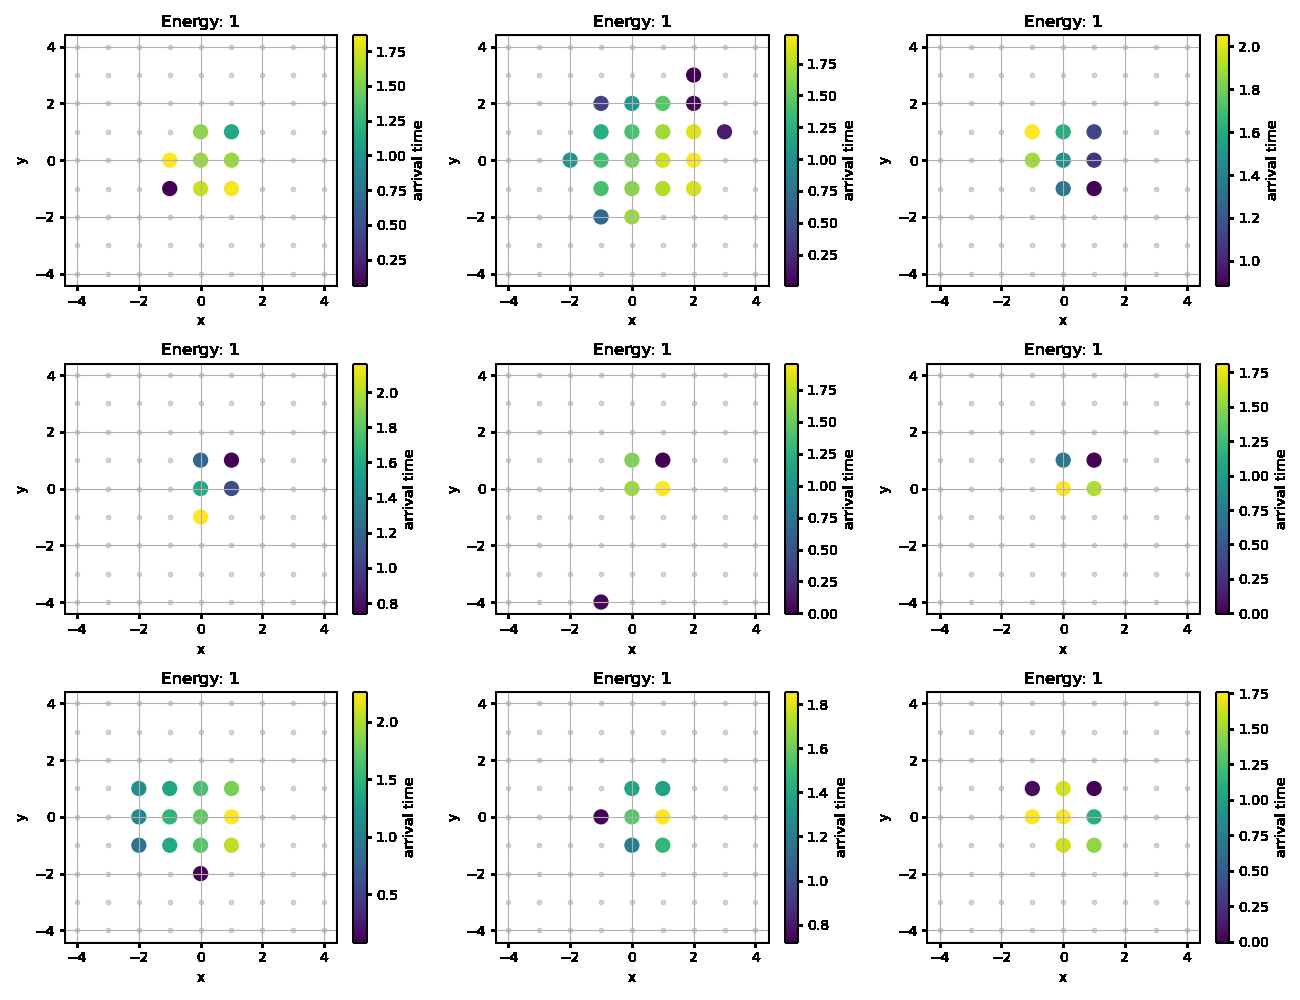
\includegraphics[width=100mm,scale=0.5]{Figures/res/CWGANGP_LD128_R0/fake.png}
    \decoRule
    \caption[Cascadas generadas 0]{
        Cascadas generadas con una vector latente con dimension 128
    }
    \label{fig:ld128r0fakeshower}
\end{figure}

Comparación con las cascadas reales (Figura ~ \ref{fig:ld128r0realshower}).

\begin{figure}
    \centering
    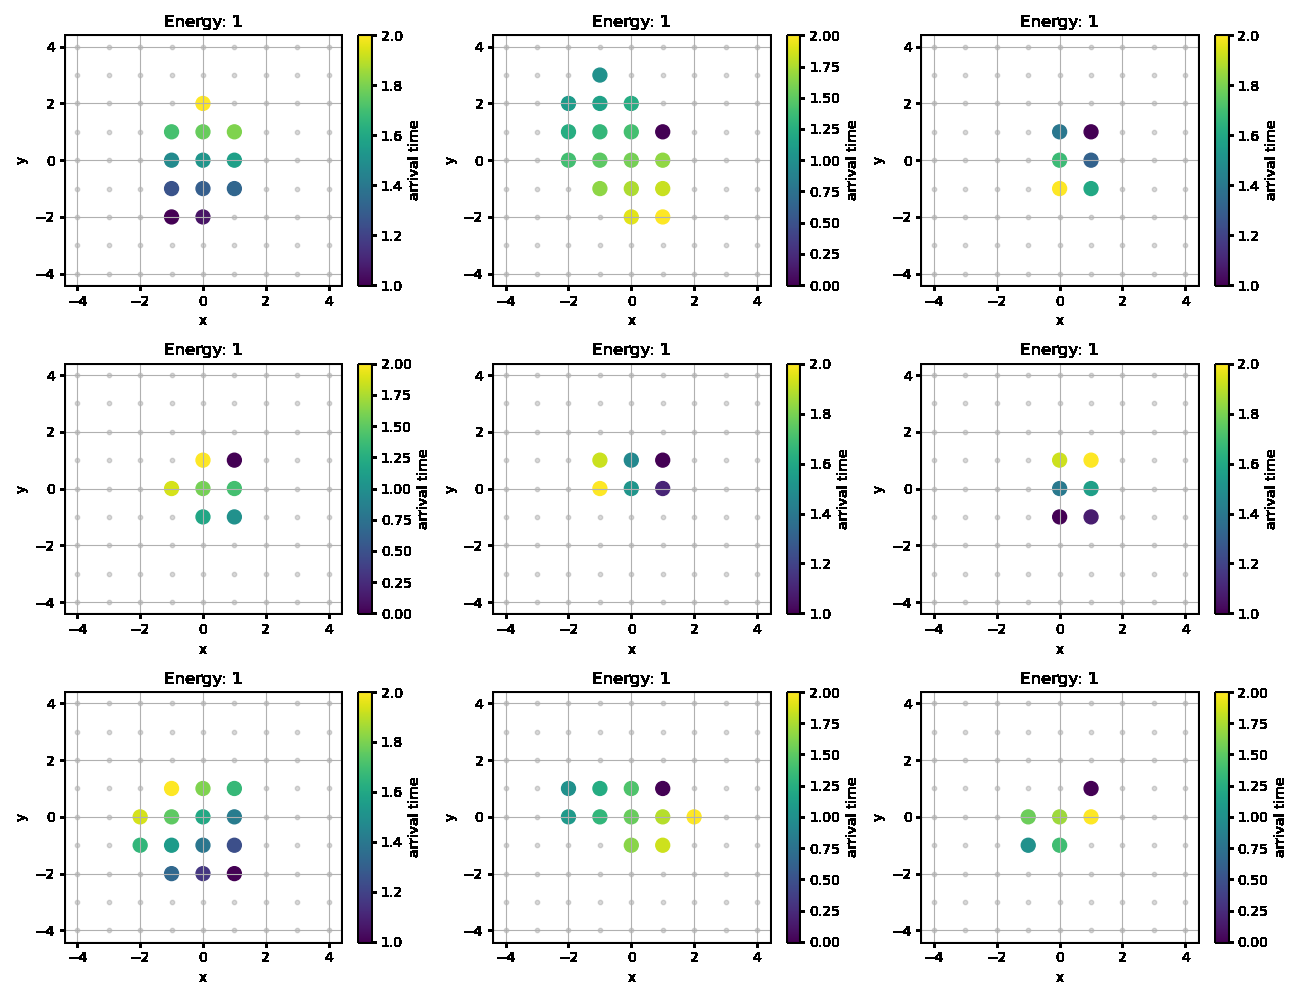
\includegraphics[width=100mm,scale=0.5]{Figures/res/CWGANGP_LD128_R0/real.png}
    \decoRule
    \caption[Cascadas reales 0]{
        Cascadas reales
    }
    \label{fig:ld128r0realshower}
\end{figure}

Perdidas de cada modelo (Figura ~ \ref{fig:ld128r0losses}).

\begin{figure}
    \centering
    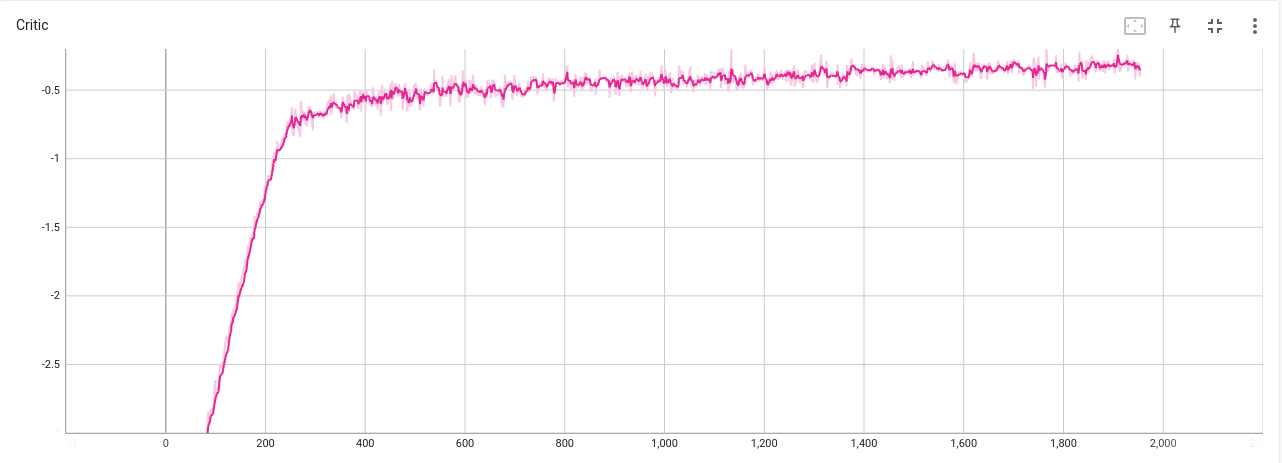
\includegraphics[width=100mm,scale=0.5]{Figures/res/CWGANGP_LD128_R0/critic.png}
    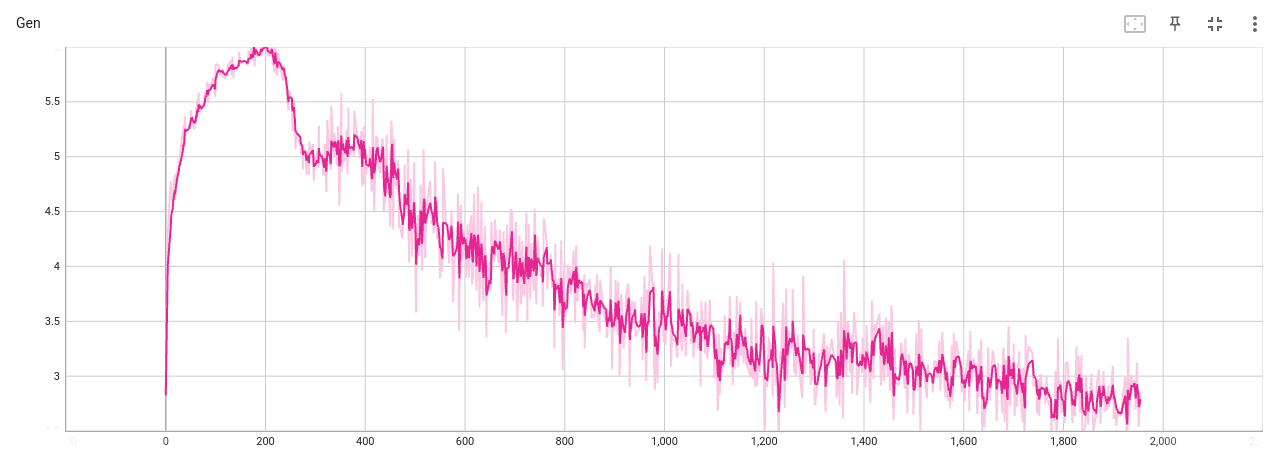
\includegraphics[width=100mm,scale=0.5]{Figures/res/CWGANGP_LD128_R0/gen.png}
    \decoRule
    \caption[Perdidas 0]{
        Funciones de perdida el modelo anterior.
    }
    \label{fig:ld128r0losses}
\end{figure}

\subsubsection*{Dimensión latente = 4}

Cascadas electromagnéticas generadas con un vector latente con dimensión de 4  (Figura ~ \ref{fig:ld4r0fakeshower}).
%\ref{tabla}
%insertar cascadas generadas.

\begin{figure}
    \centering
    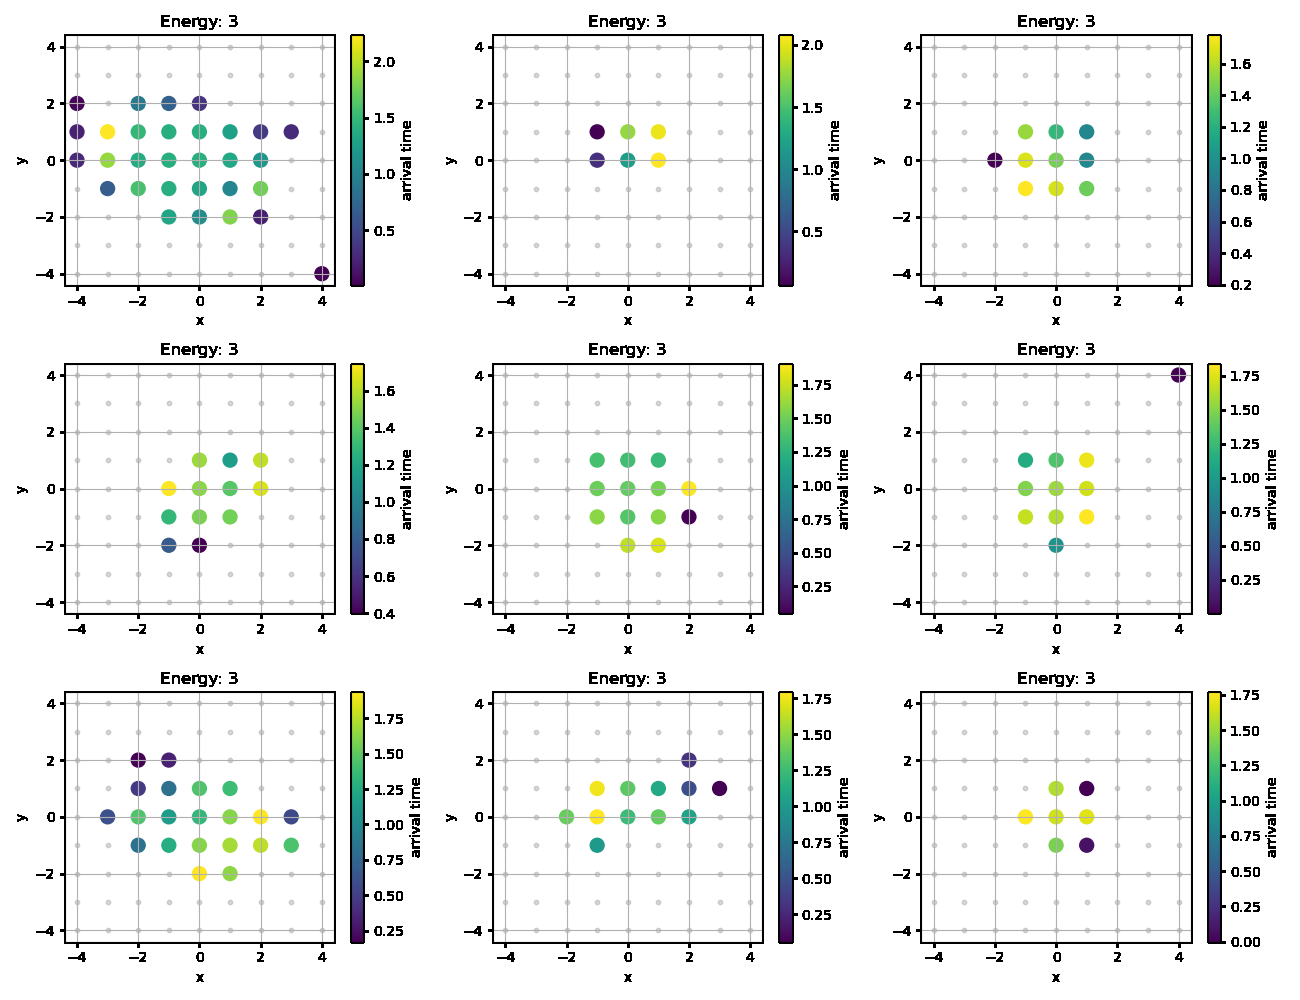
\includegraphics[width=100mm,scale=0.5]{Figures/res/CWGANGP_LD4_R4/fakestep4.png}
    \decoRule
    \caption[Cascadas generadas 1]{
        Cascadas generadas con una vector latente con dimension 4
    }
    \label{fig:ld4r0fakeshower}
\end{figure}

Comparación con las cascadas reales (Figura ~ \ref{fig:ld4r0realshower}).

\begin{figure}
    \centering
    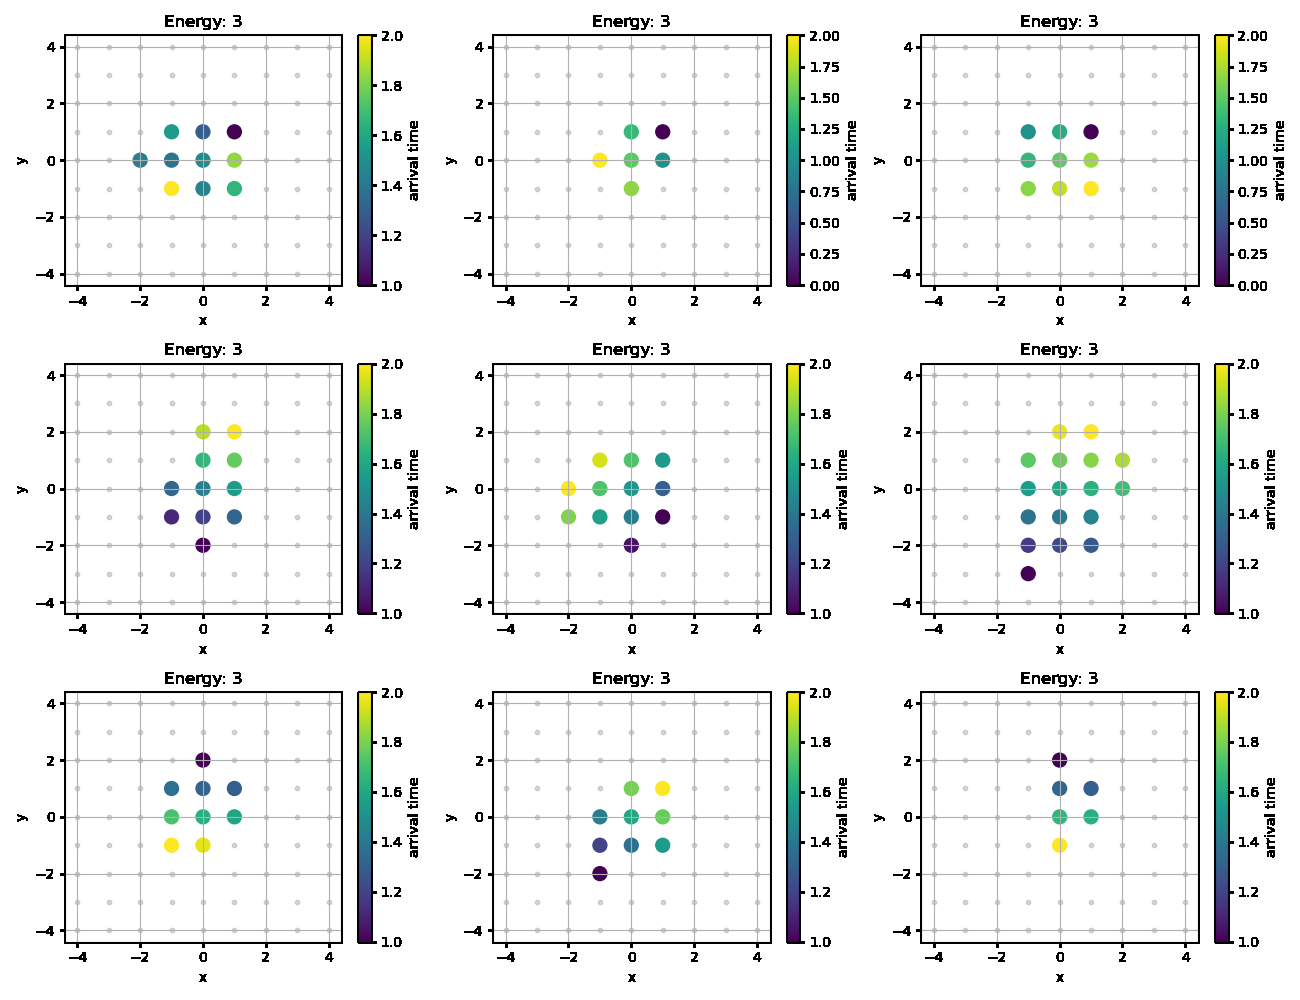
\includegraphics[width=100mm,scale=0.5]{Figures/res/CWGANGP_LD4_R4/realstep4.png}
    \decoRule
    \caption[Cascadas reales 1]{
        Cascadas reales
    }
    \label{fig:ld4r0realshower}
\end{figure}

Perdidas de cada modelo (Figura ~ \ref{fig:ld4r0losses}).

\begin{figure}
    \centering
    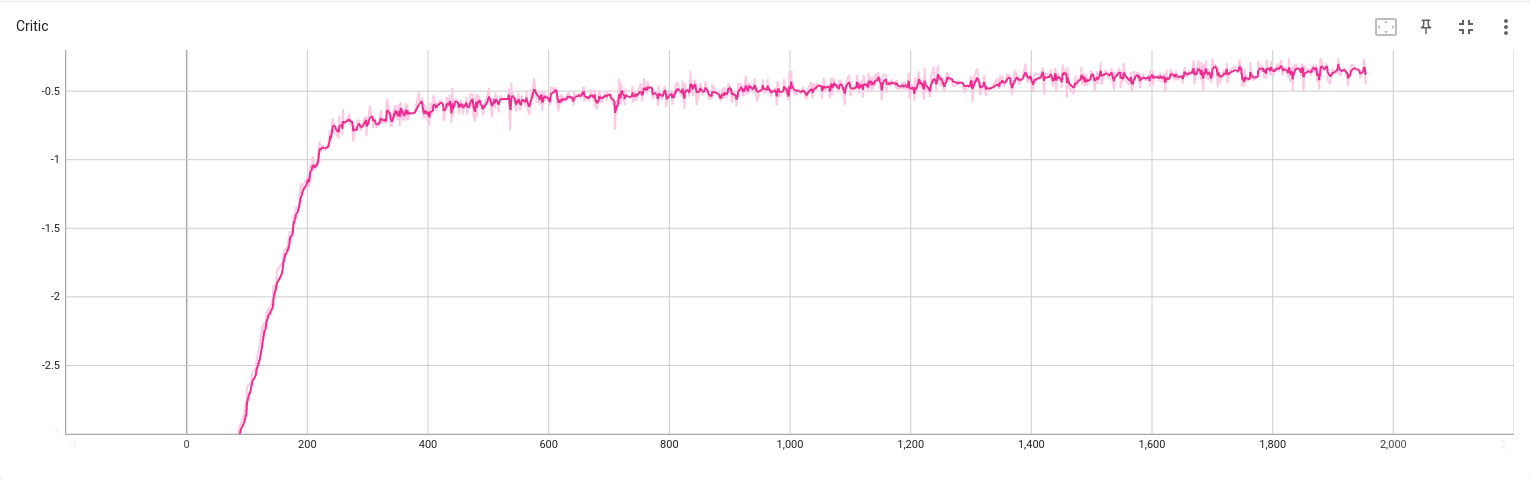
\includegraphics[width=100mm,scale=0.5]{Figures/res/CWGANGP_LD4_R4/criticloss.png}
    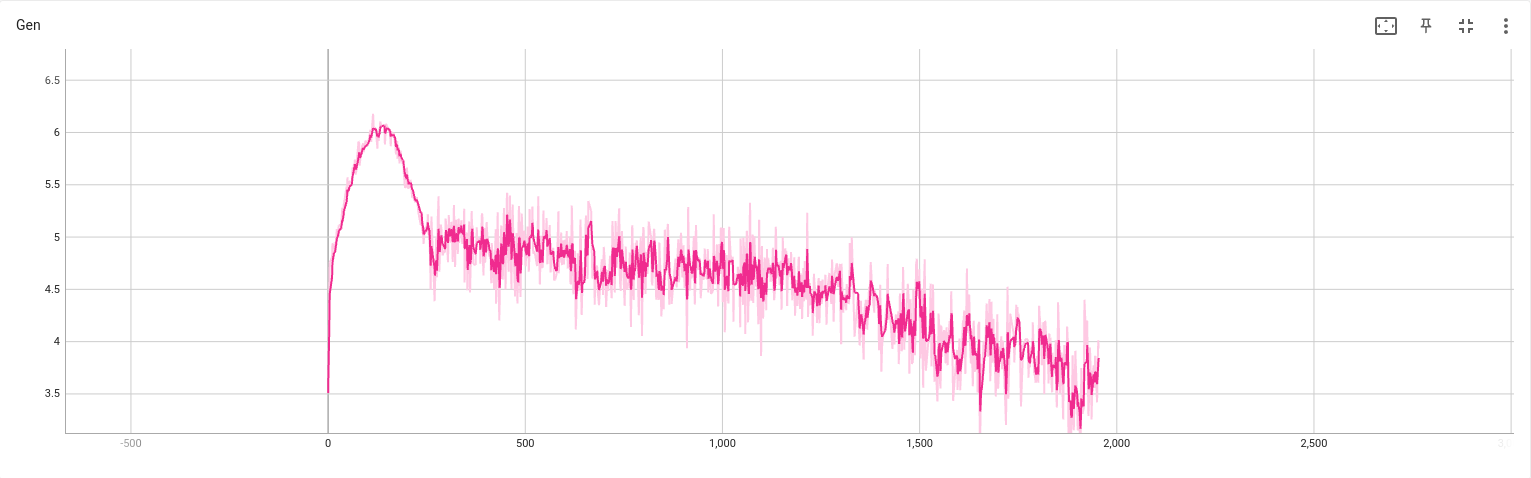
\includegraphics[width=100mm,scale=0.5]{Figures/res/CWGANGP_LD4_R4/genloss.png}
    \decoRule
    \caption[Perdidas 0]{
        Funciones de perdida el modelo anterior.
    }
    \label{fig:ld4r0losses}
\end{figure}



% \subsection*{Combinaciones lineales de vectores latentes}

% Resultados al promediar vectores latentes y hacer una combinación lineal de estos para después ser insertados en categorías energéticas diferentes.
%insertar imágenes.

% \lstinputlisting[language=Python]{Code/dfa.py}